\chapter{Implementation\label{cha:chapter4}}
The previous chapters have established a foundation for this thesis. The need for anonymization granularity in \acp{DES} has been discussed in Chapter \ref{cha:chapter1}. The existing literature and research were provided in Chapter \ref{cha:chapter2} with an emphasis on anonymization techniques specifically for streaming data. Here, Apache Kafka was also showcased as one of the leading \acp{DES}. We selected to use Kafka as the \ac{DES} in our implementation as well. Chapter \ref{cha:chapter3} served as an outline of the expected functionality of the system. This chapter on hand focuses on the practical steps taken to materialize the aforementioned system, detailing the technological choices, development processes, and the resulting product. \par
First, we evaluated the existing authentication and authorization available to users of Apache Kafka. We found that authentication is provided with the options of SSL, SASL, and Kerberos, as well as an additional option for pluggable authentication beyond that. For authorization, however, only \acp{ACL} were available. Therefore, we constructed a system attached to the administrative component of Kafka, capable of abstracting the \acp{ACL} to enable \ac{RBAC} policies. The details of this system are addressed in the first section of this chapter. Next, the focus shifts to the central component of the implementation: the \acf{DASH}. We will go in-depth on its various components, illuminate the thought process, highlight its core features, and explain how it can be adapted going forward. For effective testing of the system, a data pipeline has been constructed using the aforementioned components. To complete the pipeline we have added a Data Generator, a Kafka Connector, and a Kafka Consumer. They will be the focal point of the Data Pipeline section. Finally, the concluding section will demonstrate the integration of these components into a cohesive system, facilitated by Docker for ease of use and deployment.
\newpage

\section{Role Based Access Control}
This section presents the implementation of a system designed to enable the \acf{RBAC} policy for Apache Kafka, as directed by the Data Officer. It follows a streamlined variant of the Repository-Service-Controller software development architecture. It includes a Controller for Kafka, a \ac{CLI} for the Data Officer as well as a database - but skips the service in favor of more straightforward transactional processing. \par
Inherently, Kafka incorporates mechanisms that enforce access control on specific resources or their groups. However, the specification of policies is limited to \acp{ACL} in Kafka. Nevertheless, Kafka allows changes to these \acp{ACL} to be administered programmatically by an authenticated and authorized user. This is where our \ac{RBAC} system comes into play. \par
The system abstracts Kafka's Object-oriented access security model, realized through \acp{ACL}, transitioning it to a role-based access control paradigm. Here, the authorized permissions of actions on objects are no longer defined for subjects e.g. users, but to roles. Subsequently, roles are assigned to users, granting them the cumulative permissions associated with each assigned role. \par
Realizing this abstraction requires memory of the mappings of permissions to roles, users to roles, and overall users as well as roles. To achieve this, the \ac{RBAC} system incorporates an SQLite \cite{sqlite} database, consisting of three tables: \texttt{Users}, \texttt{Roles}, and \texttt{UserRoles}. We chose SQLite for its in-memory data storage, its simplicity in both administration and development - and its high reliability. The permissions are stored as text in the \texttt{Roles} table alongside the role name and an autoincremented unique role ID. The username is stored in the \texttt{Users} table together with an autoincremented unique user ID. This relationship is represented in the \texttt{UserRoles} table, where both role and user IDs function as foreign keys, and the combination of userId and roleId forms the primary key. This allows one user to be assigned to many roles. \par
Administrative operations are executed by the Data Officer via a \ac{CLI}, developed using the JCommander framework \cite{jcommander} and accessed through the \texttt{rbac\_cli.sh} shell script located in the system's root directory. The commands in Table \ref{table:rbac_commands} are available to the Data Officer.

\begin{table}[ht]
   \centering
   \footnotesize
   \renewcommand{\arraystretch}{1.5}
   \renewcommand\cellgape{\Gape[3.5pt]}
   \begin{tabular}{|l|l|l|}
   \hline
   \textbf{Command} & \textbf{Parameters} & \textbf{Description}\\
   \hline
   addUser & \texttt{--userName <userName>} & Adds a user \\
   \hline
   deleteUser & \texttt{--userName <userName>} & Deletes a user \\
   \hline
   addRole &  \makecell[l]{\texttt{--roleName <roleName>} \\ \texttt{--permissions <topic1,...>}}  & \makecell[l]{Adds a role with a List \\ of permissions}\\
   \hline
   deleteRole & \texttt{--roleName <roleName>} & Deletes a role\\
   \hline
   addPermission & \makecell[l]{\texttt{--roleName <roleName>} \\ \texttt{--topicName <topic>}} & \makecell[l]{Adds a permission \\ to a role}\\
   \hline
   removePermission & \makecell[l]{\texttt{--roleName <roleName>} \\ \texttt{--topicName <topic>}} & \makecell[l]{Removes a permission \\ from a role} \\
   \hline
   assignRole & \makecell[l]{\texttt{--userName <userName>} \\ \texttt{--roleName <roleName>}} & Assigns a user to a role \\
   \hline
   removeRole & \makecell[l]{\texttt{--userName <userName>} \\ \texttt{--roleName <roleName>}} & \makecell[l]{Removes a role from a \\user} \\
   \hline
   userStatus & \texttt{--userName <userName>} & \makecell[l]{Prints the roles and\\ permissions for a user} \\
   \hline
   roleStatus & \texttt{--roleName <roleName>} & \makecell[l]{Prints the permissions \\ and users for a role } \\
   \hline
   roles & \makecell[r]{-} & Lists all roles \\
   \hline
   users & \makecell[r]{-} & Lists all users \\
   \hline
   exit & \makecell[r]{-} & Exits the system \\
   \hline
   help & \makecell[r]{-} & Prints this table \\
   \hline
   \end{tabular}
   \caption{List of available commands with parameters and a description in the RBAC System.}
   \label{table:rbac_commands}
\end{table}
   
It is important to note that in this context, permissions correspond directly to topic names. The reason is that in our application solely the consumers of topics are restricted. A permission here can therefore be understood as the permissible action 'consume' for the object 'topic' by the subject 'user'. \par
The commands originate at the Data Officer, find their way into the \ac{RBAC} system through the \ac{CLI}, and are applied to the database by a dedicated database manager. When changes to the database are made, the database manager also looks for changes in permission in the database before and after the transaction. If there are changes, these get forwarded to a separate controller - named \texttt{KafkaController}. Here, the changes arrive in the form of two parameters - a HashMap of Strings (user name) and List of Strings (permissions) as well as a boolean (whether constructive or destructive change). These are then transformed into \acp{ACL} and forwarded to Kafka. \par
To establish a connection with Kafka's administrative interface, capable of realizing changes on the Kafka server, specific configurations are mandated. First, authorization and authentication must be enabled. Note how this is not the default behavior of Apache Kafka. Additionally, access control lists are enabled in Zookeeper to enact the access control mechanisms within Kafka. There are different authentication techniques available including Kerberos, SSL, and \ac{SASL}. We opted for \ac{SASL} plaintext authentication for simplicity. Each Client and Server in the Kafka network then must provide a \ac{JAAS} configuration file to authenticate against the network. These are included in the run scripts of both Zookeeper and the Kafka Server as well as all Clients. The \ac{JAAS} configuration files crucially include username and password for the network. Furthermore, the user specified in the \ac{JAAS} configuration file of the \ac{RBAC} system must be registered as a superuser in the server properties of Kafka to be allowed to administer \ac{ACL} changes. \par
With proper authentication and authorization in place, role-based access control can effectively be facilitated seemingly straightforwardly by the Data Officer for Apache Kafka.




\section{DASH - Data Anonymization Stream Handler\label{sec:dash}}
Integral to the system is the anonymization of the data stream. This led to the conceptualization of the Anonymization Stream Factory, as introduced in Section \ref{sec:model_architecture}. Its main tasks are threefold: First, it must understand the anonymization granularity relayed in the requirements input by the user. Second, it must apply these requirements to separate anonymized streams. Third, it must provide an interface to monitor and manipulate the streams. Additionally, the success of this component is critically dependent on its reliability, adaptability, and performance. To fulfill these tasks, the \acf{DASH} was developed. The following subsection will provide a comprehensive analysis of \ac{DASH}, addressing its functionalities, interactions, and thought processes that went into its development. \ac{DASH} was developed with Java (Version 11), selected due to Kafka's implementation in Java, thus offering more comprehensive and up-to-date support. A UML Class Diagram was created and will assist in explaining the implementation. It can be found in full in Figure \ref{fig:full_class_diagram} in Appendix A. However, as it spans multiple pages, we will only include excerpts of it in the subsections. 

\subsection{Overview of Anonymization Techniques}
In chapter \ref{cha:chapter2} we have detailed various anonymization techniques. In the subsequent chapter \ref{cha:chapter3} we have categorized them into more comprehensible groups. Based on that we have implemented the vast majority of anonymization techniques and made them available in \ac{DASH}. They are elaborated in Table \ref{table:anonymizer_parameters}. The anonymization techniques are color-coded to show their corresponding anonymization category. Each anonymizer needs some parameters specified for configuration, these are detailed in the table as well. This includes their format or type, whether they are required for the configuration or optional, and a short description of the parameter. Among the value-based anonymization techniques, highlighted in blue, we implemented all but one in \ac{DASH}, Tokenization. Tokenization requires a database as an input parameter and the development overhead for the creation, validation, and testing of such a database was not in the scope of this thesis.\par 
The green highlighted tuple-based anonymization technique conditional substitution is included in \ac{DASH}. This technique supports three distinct kinds of conditions: value matches, numerical ranges, and regular expressions, thereby enhancing its versatility in application.\par 
The red highlighted implemented attribute-based anonymization techniques include Aggregation, its specialization Univariate Microaggregation, and Shuffling. As attribute-based anonymization techniques, they operate on a collection of tuples. \ac{DASH} creates discrete sets of tuples by cutting up the data stream, a technique called windowing. Kafka supports this inherently. There are different kinds of windows available. \ac{DASH} can be configured to work with different kinds of windowing techniques per anonymization stream. The available window types are tumbling and sliding. Both are fixed size, as specified by the required windowSize parameter. Sliding in comparison to tumbling allows the overlapping of windows. A tuple in a sliding window can therefore be included in more than one window, whereas in a tumbling window, it can only be included in one. By setting only the windowSize parameter, the user specifies the window size of a tumbling window. The specification of the optional advance time turns that into a sliding window that moves along the time axis according to that parameter, creating new windows for every advance time unit. Additionally, a grace period can optionally be set. As data streams operate in real-time tuples can be delayed in their transition to the system. A late-arriving tuple can be identified by its associated timestamp and stream position. If the grace period is specified a window waits that amount of time before forwarding the tuples to processing to allow for latecomers to be included. Grace periods are available for both tumbling and sliding windows. These window configurations apply to all attribute-based anonymization techniques. \par 
Aggregation and Univariate Microaggregation operate on numerical attributes and aggregate the attributes specified in the 'keys' parameters within a window. Aggregation offers various modes: sum, median, average max, min, count, and mode. It replaces the values of these attributes with the computed values of the specified modes (count refers to the number of tuples within the window; mode refers to the most frequent value within the window). The Univariate Microaggregation is implemented as detailed in Algorithm \ref{algo:uniMicroAgg}. Shuffling can be additionally configured with a seed, making it deterministic. In the case that there are multiple keys to shuffle it can both shuffle them together, ensuring that the content of these attributes remain together after the shuffle, or independently. \par
Finally, the table-based anonymization technique is highlighted in yellow. It includes the implementation of CASTLE's k-anonymization as specified in \ref{lit:castle}. Here, the tuples are processed one at a time instead of windowed as in the attribute-based anonymization techniques. Even though they are entering \ac{DASH} one at a time, they are grouped in static clusters and are only released after expiration as determined by the delta parameter in CASTLE. The implementation requires the Data Officer to specify multiple parameters. Most are simply positive integers defining different aspects of the algorithm. Additionally, the attributes containing \ac{PII} are included to be suppressed. Finally, the quasi-identifiers have to be specified. Remember, these are the attributes that the k-anonymization is applied to. Any set of k entries in the output stream must be indistinguishable concerning their quasi-identifiers. These are generalized and not suppressed to minimize information loss. The 'quasiIdentifiers' parameter is a List containing a String and GeneralizationHierarchy for each quasi-identifier. The String is the attribute name. The 'GeneralizationHierarchy' is a special data structure designed for the implementation of CASTLE. It can take on two forms for the two types of attributes - numerical and categorical. A numerical generalization is specified through a numerical range as well as the bucket size and in its generalization logic equals bucketizing. The categorical attribute requires a generalization tree. Each node has two attributes - the value, e.g. the generalization of that node, and its children, e.g. an array of nodes. \ac{DASH} then applies the algorithms described in CASTLE. The extension to l-diversity was not implemented in \ac{DASH}, but it already provides the bulk of the code necessary including various data structures and methods. However, it was not within the scope of this thesis. Similarly, further extensions to facilitate t-closeness were also excluded from the scope of this thesis. It was decided against implementing Multivariate Microaggregation as there is no optimal algorithm available at this time. 

\setlength{\LTleft}{-40pt}    
\setlength{\LTright}{-20pt} 
\begin{footnotesize}
   \renewcommand{\arraystretch}{1.5}
   \captionsetup{font=normalsize}
      \begin{longtable}{|C{2.5cm}|C{2.5cm}|C{2.5cm}|C{2.5cm}|C{1.6cm}|L{3.5cm}|}
         \caption{
            List of Anonymizers available in the \acf{DASH}. 
            They are listed with their respective category color coded as well as their parameters including the parameter type and whether it is required or not. 
            A description of the parameters is also added.\label{table:anonymizer_parameters}
         } \\
         \hline
         \textbf{Category} & \textbf{Anonymizer} & \textbf{Parameter} & \textbf{Type} & \textbf{Required} & \multicolumn{1}{c|}{\textbf{Description}} \\
         \hline
         \endfirsthead
         \multicolumn{6}{c}%
         {\tablename\ \thetable\ -- \textit{Continued from previous page}} \\
         \hline
         \textbf{Category} & \textbf{Anonymizer} & \textbf{Parameters} & \textbf{Type} & \textbf{Required} & \multicolumn{1}{c|}{\textbf{Description}} \\
         \hline
         \endhead
         \hline \multicolumn{6}{r}{\textit{Continued on next page}} \\
         \endfoot
         \hline
         \endlastfoot

         \cellcolor{lightblue} ValueBased & Blurring & keys & List\textless String\textgreater & \checkmark & List of attribute names to blur\\
         \cline{3-6}
         \cellcolor{lightblue} & & nFields & positive integer & $\times$ & Number of fields to blur \\
         \cline{2-6}
         \cellcolor{lightblue} & Bucketizing & keys & List\textless String\textgreater & \checkmark & List of attribute names to bucketize\\ 
         \cline{3-6}
         \cellcolor{lightblue} && bucketSize & positive integer & \checkmark & Size of each bucket \\
         \cline{2-6}
         \cellcolor{lightblue} & Generalization & keys  & List\textless String\textgreater & \checkmark & List of attributes to generalize \\
         \cline{3-6}
         \cellcolor{lightblue} && generalization\-Map & HashMap\ \textless String, String\textgreater & \checkmark & Generalization for each value \\
         \cline{2-6}
         \cellcolor{lightblue} & NoiseMethods & keys & List\textless String\textgreater & \checkmark & List of attributes to apply noise \\
         \cline{3-6} 
         \cellcolor{lightblue} && noise & positive double & \checkmark & Amount of Noise; typically between 0 and 1 \\
         \cline{2-6}
         \cellcolor{lightblue} & Substitution & keys & List\textless String\textgreater & \checkmark & List of attributes to substitute \\
         \cline{3-6}
         \cellcolor{lightblue} && substitutionList & List\textless String\textgreater & \checkmark & List of substitutes \\
         \cline{2-6}
         \cellcolor{lightblue} & Suppression & keys & List\textless String\textgreater & \checkmark & List of attributes to suppress \\
         \hline
         \cellcolor{lightgreen} TupleBased & Conditional Substitution & keys & List\textless String\textgreater & \checkmark & List of attributes to substitute \\
         \cline{3-6}
         \cellcolor{lightgreen} && condition\-Map & HashMap\ \textless String, Object\textgreater & \checkmark & Conditions mapped to the attribute they correspond to. Conditions can be of three different formats: value matches, numerical ranges, and regular expressions \\
         \hline
         \cellcolor{lightred} AttributeBased & Aggregation & keys & List\textless String\textgreater & \checkmark & List of attributes to aggregate \\
         \cline{3-6}
         \cellcolor{lightred} && aggregation\-Mode & String & \checkmark & Type of numerical aggregation performed on the values. The options are "sum", "median", "average", "max", "min", "count" and "mode" \\
         \cline{3-6}
         \cellcolor{lightred} && windowSize & positive integer & \checkmark & Duration of a window in ms. \\
         \cline{3-6}
         \cellcolor{lightred} && advanceTime & positive integer & $\times$ & Duration of the window's advance time in ms. \\
         \cline{3-6}
         \cellcolor{lightred} && gracePeriod & positive integer & $\times$ & Duration of the window's grace period in ms. \\
         \cline{2-6}
         \cellcolor{lightred} & Shuffling & keys & List\textless String\textgreater & \checkmark & List of attributes to shuffle \\
         \cline{3-6}
         \cellcolor{lightred} && seed & positive integer & $\times$ & Specify the randomizing seed. \\
         \cline{3-6}
         \cellcolor{lightred} && shuffle\-Individually & boolean & $\times$ & Shuffle the specified attributes individually or collectively e.g. disrupt the correspondence of the attributes that are shuffled. \\
         \cline{3-6}
         \cellcolor{lightred} && windowSize & positive integer & \checkmark & Duration of a window in ms. \\
         \cline{3-6}
         \cellcolor{lightred} && advanceTime & positive integer & $\times$ & Duration of the window's advance time in ms. \\
         \cline{3-6}
         \cellcolor{lightred}  && gracePeriod & positive integer & $\times$ & Duration of the window's grace period in ms. \\
         \cellcolor{lightred} & Univariate\ Micro\-aggregation & keys & List\textless String\textgreater & \checkmark & List of attributes to microaggregate. They will be aggregated individually as this is univariate \\ 
         \cline{3-6}
         \cellcolor{lightred} && k & positive integer & \checkmark & Number of minimal observations per subgroup \\
         \cline{3-6}
         \cellcolor{lightred} && windowSize & positive integer & \checkmark & Duration of a window in ms. \\
         \cline{3-6}
         \cellcolor{lightred} && advanceTime & positive integer & $\times$ & Duration of the window's advance time in ms. \\
         \cline{3-6}
         \cellcolor{lightred} && gracePeriod & positive integer & $\times$ & Duration of the window's grace period in ms. \\
         \cline{2-6}
         \hline
         \cellcolor{lightyellow} TableBased & K\-Anonymization & keys & List\textless String\textgreater & \checkmark & List of attributes to suppress e.g. \ac{PII} \\
         \cline{3-6}
         \cellcolor{lightyellow} && quasiIdentifiers & List\textless String, GeneralizationHierarchy\textgreater & \checkmark & List of quasi-identifiers with their attribute and corresponding generalization hierarchy structured as a tree \\
         \cline{3-6}
         \cellcolor{lightyellow} && k & positive integer & \checkmark & Number of tuples indistinguishable in regard to their quasi identifiers \\
         \cline{3-6}
         \cellcolor{lightyellow} && delta & positive integer & \checkmark & Number of subsequent tuples until expiration \\
         \cline{3-6}
         \cellcolor{lightyellow} && mu & positive integer & \checkmark & Number of output clusters that define the average information loss parameter $\tau$ within CASTLE \\
         \cline{3-6}
         \cellcolor{lightyellow} && beta & positive integer & \checkmark & Maximum amount of clusters \\
         \hline 
      \end{longtable}
\end{footnotesize}

Internally, \ac{DASH} categorizes the anonymizers with the usage of interfaces. There are four distinct interfaces, one for each of the four anonymization categories. Then there is the overarching Anonymizer interface, which dictates all anonymizers. This interface mandates the implementation of four methods. The primary method, \texttt{anonymize(lines : List<Struct>)}, feeds input data streams to the anonymizers and yields the anonymized output. The \texttt{Struct} data structure is what \ac{DASH} uses internally. It is Kafka native and is similar to a tuple in that it splits the tuple into its attributes, which can be accessed and modified in place through its indices as well as the attribute name. The latter is what \ac{DASH} uses primarily and which is the reason it requires the List of attributes as the anonymizer parameters. Alternatively, indices could have been used synonymously. Note, value, and tuple-based anonymizers receive and return only one tuple at a time, attribute-based receive and return collections of tuples, and table-based receive one tuple at a time but return empty lists or collections of tuples courtesy of CASTLE. Owing to these semantic variations, \ac{DASH} necessitates that anonymizers within the same stream belong to the same category. The anonymizers are connected in series so the output of one anonymizer will be the input of the next. If their semantics were different, this would not work. To ensure category compliance the anonymizer interface requires the implementation of the \texttt{getAnonymizationCategory()}. This method is not implemented by any anonymizer - but defaulted by their category interface. This validation process is handled by the stream configuration builder, a component that will be discussed in greater detail later in this section. For further validation, the anonymizer interface includes the method \texttt{getParameterExpectations()}. Each anonymizer relies on different specific parameters that need or can be configured before runtime. These are specified in their implementations together with validation logic syntactically and semantically validating the input configuration. How this works will also be addressed in-depth in the subsequent subsections. The anonymizers are made available through a static class \texttt{AnonymizerRegistry}. It includes a HashMap of all anonymizer names and their classes. From here, the stream configuration builder can get access to the anonymizers' methods, validate them, and ultimately with their last method \texttt{initialize(parameters : List<Parameter>)} configure them. This structure was designed to facilitate further adaptations. To include a new anonymizer the developer has to decide on an anonymization category and create a class implementing the corresponding interface. The inclusion of the anonymizer's name and class in the registry completes this integration process. From then on it will be available in \ac{DASH}.


\subsection{Parsing and Analysis of Anonymization Requirements\label{sec:json_loader}}
This subsection begins with a dissection of the anonymization requirements, made up of two distinct components: the underlying data stream and the anony\-miza\-tion granularity built upon it. Together they contain all information necessary for the anonymization process. The requirements are encapsulated in a JSON file format. We chose JSON because of its widespread use and familiarity among technical users. JSON's format, with its ability to handle attribute-value pairs and arrays, allows efficient parsing and representation of the requirements. Code Fragment \ref{code:requirements} shows an exemplary configuration setup. 

\begin{lstlisting}[language=json, captionpos=b, caption={Example JSON Configuration for DASH. The \textit{globalConfig} specifies the underlying data stream. The \textit{Schema} refers to either an \textit{AVRO} or \textit{KAFKA\_STRUCT} data schema. Each entry in the \textit{streamProperties} defines an anonymized version of the original data consisting of a list of \textit{anonymizers}.}, breaklines=true, basicstyle=\ttfamily\footnotesize, frame=tb, label=code:requirements]
{
      "globalConfig": {
         "bootstrapServer": "STRING",
         "topic": "STRING",
         "dataSchema": "AVRO" or "KAFKA_STRUCT"
      },
      "streamProperties": [
         {
            "applicationId": "STRING",
            "category": "ENUM (VALUE_BASED, TUPLE_BASED, ATTRIBUTE_BASED, TABLE_BASED)",
            "anonymizers": [
                  {
                     "anonymizer": "STRING (suppression, substitution, etc.)",
                     "parameters": [
                        {
                              "keys": [
                                 "key": "STRING"
                                 // ... other keys
                              ],
                              // ... other parameters
                        }
                     ]
                  },
                  // ... other anonymizers
            ]
         },
         // ... other stream configs
      ]
}
\end{lstlisting}
   
We named the first component global config as it includes valuable information for all streams. The bootstrap server, defined as the IP address of the Kafka server, the topic is the unique name of the stream that is to be anonymized - both are strings. The data schema, highlighted in green, defines the attributes and types of the data within the stream. Here, \ac{DASH} supports two data schema types: Kafka Struct and Avro. They are among the most popular schemas in use for Kafka. For the use case example of Section \ref{sec:anon_granularity} the schemas would be defined as shown in Figure \ref{fig:avro_kafkastruct_schemas}. 

\begin{figure}[ht]
   \centering
   \begin{minipage}{.45\textwidth}
     \begin{lstlisting}[language=json, basicstyle=\ttfamily\notsotiny, frame=tb]
 {
   "type": "AVRO",
   "name": "Patient",
   "fields": [
     {"name": "pid", "type": "int"},
     {"name": "name", "type": "string"},
     {"name": "zip", "type": int},
     {"name": "sex", "type": string},
     {"name": "age", "type": int},
     {"name": "ins. co.", "type": string},
     {"name": "ins. no.", "type": string},
     {"name": "diag.", "type": string},
     {"name": "gluc.", "type": double},
     {"name": "hba1c", "type": double},
     {"name": "med.", "type": string}
   ]
 }
     \end{lstlisting}
   \end{minipage}\hfill
   \begin{minipage}{.45\textwidth}
     \begin{lstlisting}[language=json, basicstyle=\ttfamily\notsotiny, frame=tb]
 {
   "type": "KAFKA_STRUCT",
   "fields": [
     {"field": "pid", "type": "int32"},
     {"field": "name", "type": "string"},
     {"field": "zip", "type": int32},
     {"field": "sex", "type": string},
     {"field": "age", "type": int16},
     {"field": "ins. co.", "type": string},
     {"field": "ins. no.", "type": string},
     {"field": "diag.", "type": string},
     {"field": "gluc.", "type": double32},
     {"field": "hba1c", "type": double32},
     {"field": "med.", "type": string}
   ]
 }
     \end{lstlisting}
   \end{minipage}
   \caption{Code Examples for Avro (left) and Kafka Struct (right) schemas for the patient use case.\label{fig:avro_kafkastruct_schemas}}
 \end{figure}

The second component of the requirements file details the different anonymized streams. The array can include any number of elements but must not be empty. Each stream is given an 'applicationId' equalling a name. This is important - because the combination of the original topic name with applicationId is the topic name of the resulting data stream. Next, the stream is associated with a category. Remember, in Section \ref{sec:anonymization_hierarchy} all anonymization techniques were categorized. An individual anonymized stream will only be allowed to contain anonymizers falling into that category. This addition to the requirements is mainly there to remind the user, the Data Officer, to remain in one category. It is optional and can be inferred by the system based on the rest of the stream property. Then come the anonymizers. Each is specified with a name and equipped with parameters. The list of available anonymizers and their respective parameters can be found in Table \ref{table:anonymizer_parameters}. Extensive documentation, as well as exemplary requirements, can be found alongside all other artifacts, the codebase, and the thesis itself under \url{https://github.com/TheRealHenri/master_thesis}. \par
Next, let us look at how \ac{DASH} parses and transforms the requirements. Figure \ref{fig:requirements_parser} shows the part of \ac{DASH}'s Class Diagram responsible for this task.\par

We have included similar color coding as in the Configuration in Code Fragment \ref{code:requirements} to assist in its comprehensibility. Classes with the same color signify close relations. At the very bottom of the Diagram is the connection to the rest of \ac{DASH} with the \texttt{JSONLoader}. \ac{DASH} will always put the requirements in the same file location, which is identical to the path in the \texttt{JSONLoader}, which is why the \texttt{JSONLoader} is static and does not need to be instantiated. In this process, Jackson is employed to parse the JSON. Jackson is a high-performance JSON processor for Java. It is specifically potent at creating Java Objects with the same hierarchy and types as the JSON file. This is the reasoning behind the structure of the \texttt{SystemConfiguration}. Additional logic was implemented to check for a change in the JSON file. Here, the checksum of the file is calculated and compared with the one found in the cache. If it is the same, the old \texttt{SystemConfiguration}, also cached, can be returned as no changes have occurred. Should there be any changes, or in the absence of a cached SystemConfiguration, Jackson tries to parse the JSON. It consists of two components, the \texttt{GlobalConfig} (highlighted in red in the Diagram) and the \texttt{StreamProperties} (highlighted in orange). The \texttt{GlobalConfig} includes the \texttt{DataSchema} (highlighted in teal) alongside the bootstrap server and topic identifier. The Kafka Server information together with the topic identifier uniquely specifies the underlying anonymized stream. Collectively, these elements uniquely identify the stream to be anonymized and delineate its attributes and (de-)serialization process. The \texttt{DataSchema} specifies the attribute type and attribute name pairs that make up the schema of a data stream. There are various data schema formats available and did not want to limit \ac{DASH} to a single one. Instead, \ac{DASH} abstracts data schemas into an internally used \texttt{SchemaCommon} simply containing the data fields as a HashMap. The available types are maintained in the \texttt{FieldType} Enum and include String, Int, Long, Float, Double, Boolean, and Optional values. This abstraction is achieved by implementing the \texttt{DataSchema} interface. It forces a new data schema to implement the conversion of its schema into a \texttt{SchemaCommon}. Further, it must provide the structure to be deserialized by Jackson. \ac{DASH} already provides two implementations of the \texttt{DataSchema} interface, Avro (highlighted in blue) and Kafka Struct (highlighted in purple). This should already cover most of the use cases and should further serve as examples if in the future another data schema is to be added. The deserialization of both schemas is straightforward for Jackson with the provided helper classes breaking down their hierarchies. The only difficulty lies in the types available for Avro as these include single as well as multiple types for one attribute. An additional deserializer (highlighted in green) was implemented to accomplish this task for Jackson.\par

\begin{figure}[H]
   \begin{adjustbox}{center}
   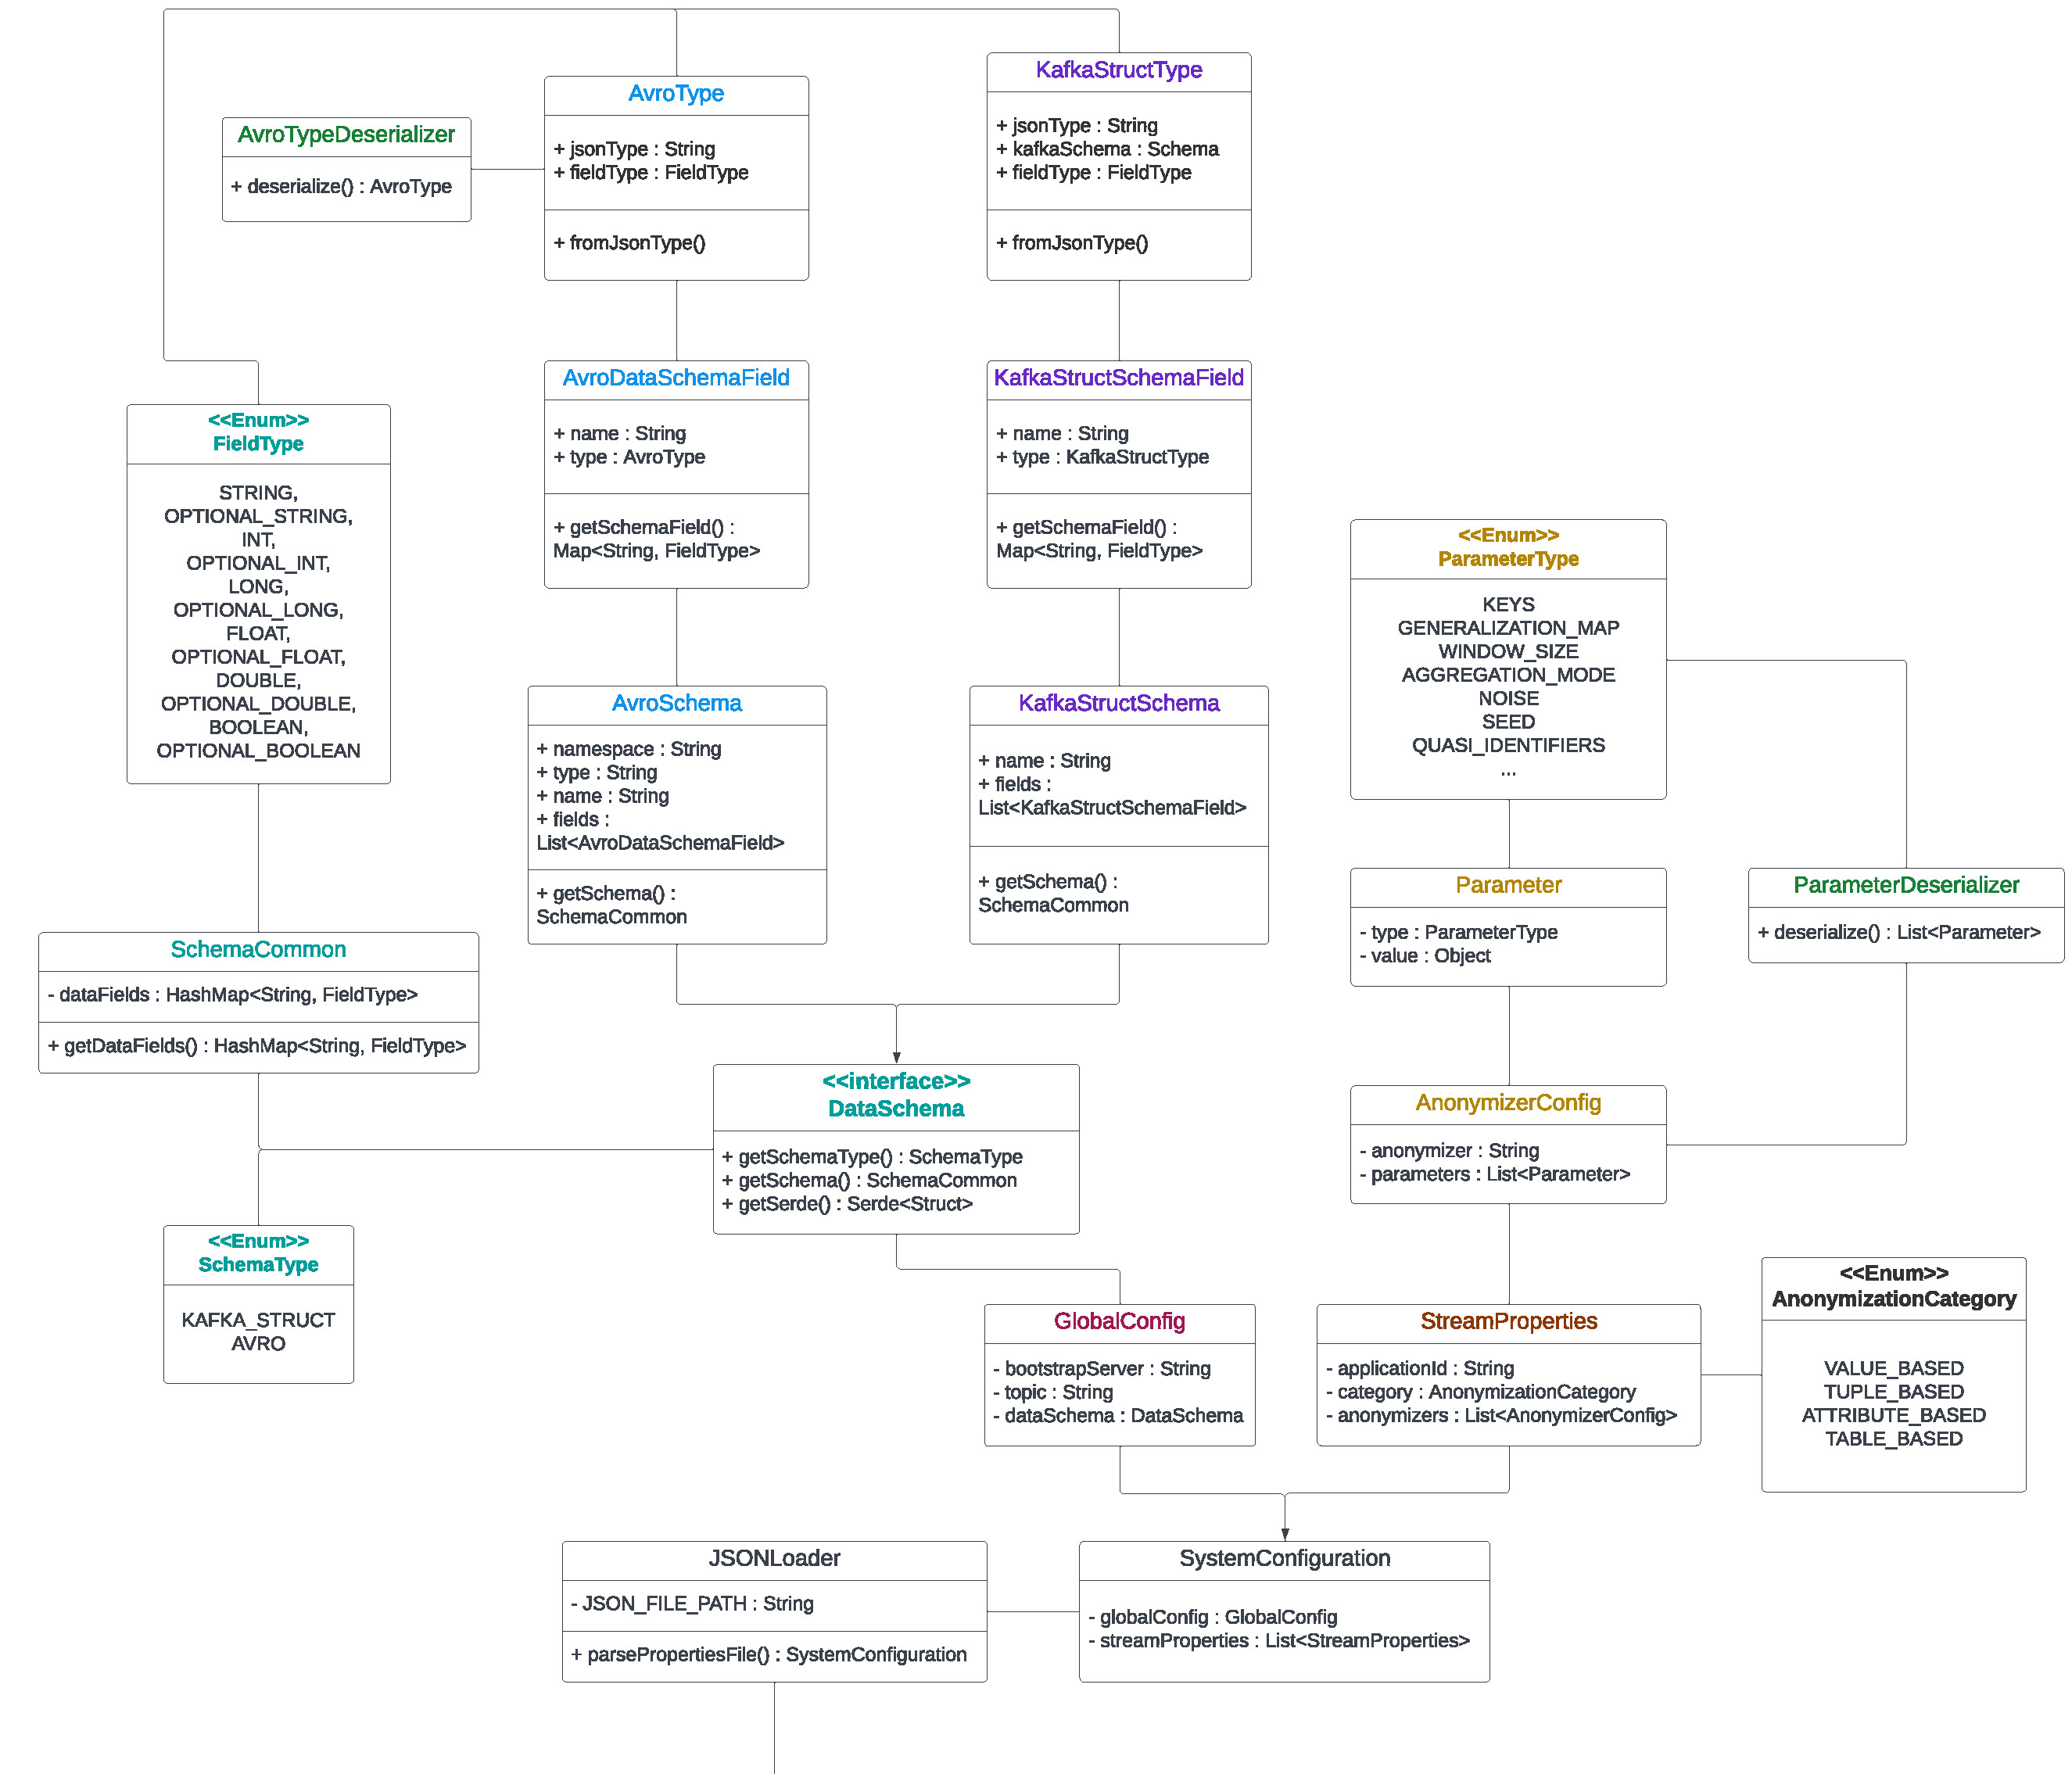
\includegraphics[width=0.85\pdfpagewidth]{img/Requirements_Parser_Class_Diagram.pdf}
   \end{adjustbox}
   \caption[Class diagram of the requirements parsing component of \ac{DASH}]{Class diagram of the JSON Loader responsible for parser the Data Officer's requirements. It connects on the bottom to the rest of \ac{DASH}. The full diagram can be found in the Appendix in Figure \ref{fig:full_class_diagram}\label{fig:requirements_parser}}
\end{figure}

Next to the \texttt{GlobalConfig} are the \texttt{StreamProperties}. Each stream includes at least one anonymizer. An anonymizer (highlighted in yellow) is specified with a name and its parameters. All available parameters of all anonymizers are represented as a constant in the \texttt{ParameterType} enum. As one anonymizer can include many parameters of different types a special \\ \texttt{ParameterDeserializer} was implemented. This deserializer processes each parameter in the list individually, converting it into an object as defined by the Parameter class corresponding to that ParameterType. These include simple types like double or int, but can simultaneously be more complex as hierarchies, enums, hashmaps, and lists. Again, \ac{DASH} has been designed to facilitate change. Adding new Parameters is as simple as adding a new value to the ParameterType enum and implementing its deserialization in the \texttt{ParameterDeserializer}.\par
The deserialization relies heavily on the correct format of the requirements and thus provides extensive error messages to the user, the Data Officer, upon failures. Additionally, a recipe with examples as well as documentation - is included in the artifacts found in the thesis repository (\url{https://github.com/TheRealHenri/master_thesis}). Consequently, the \texttt{JSONLoader} accomplishes another crucial task alongside the processing of the configuration, it checks the syntax of the requirements JSON. The deserialization accepts only the expected types for all classes and parameters. A wrong input syntactically will be caught here. The semantics of the requirements, specifically of the parameters, are validated in another component of \ac{DASH} responsible, which we will turn our attention to next. 

\subsection{Stream Config Validation and Construction\label{sec:config_builder}}
The \texttt{Stream Config Validation and Construction} aspect of DASH serves a fundamental role in preparing stream data for Kafka. It starts by taking \\ \texttt{StreamProperties} and methodically converting them into a Kafka-compatible configuration. This step involves not just creating configurations but also ensuring that each anonymizer's parameters undergo a strict validation process before they are used. The accompanying Class Diagram, shown in Figure \ref{fig:stream_config_builder}, outlines this essential process, with the functionality responsible for validation marked in teal and the functionality responsible for construction marked in red. \par

The central component is the \texttt{AnonymizationStreamConfigBuilder}, shown on the left in the figure. Algorithm \ref{algo:buildAnonymizationStreamConfig} shows pseudocode for its one method - \texttt{build(streamProperties)}. 

\begin{algorithm}[ht]
   \SetAlgoLined
   \SetKwInOut{Parameter}{Parameter}
   \SetKwInOut{Output}{Output}
   \Parameter{StreamProperties}
   \Output{Configuration for Kafka Streams}
   
   Validate StreamProperties \\
   
   \( anonymizationCategory \) ← null \\
   \( anonymizers \) ← Instantiate Anonymizers \\
   \ForEach{anonymizer}{
      \eIf{anonymizationCategory == null}{
         \( anonymizationCategory \) ← \( anonymizer \)'s anonymization category \\
      }{
         Validate \( anonymizationCategory \) \\
      }
      \( parameterExpectations \) ← \( anonymizer \)'s parameter expectations \\
      \ForEach{parameterExpectation}{
         \( parameterValidators \) ← \( parameterExpectation \)'s validators \\
         \ForEach{validator}{
            Validate Parameter
         }
      }
   }
   Initialize Anonymizers with their validated parameters\\

   \If{anonymizationCategory == ATTRIBUTE\_BASED}{
      Validate WindowConfig
   }

   \Return{new AnonymizationStreamConfig with Application ID, anonymizers list, and anonymizationCategory} \\
   \caption{Pseudocode for Building Stream Configurations}
   \label{algo:buildAnonymizationStreamConfig}
\end{algorithm}

The config builder first validates the input \texttt{StreamProperties} by checking whether an application ID for the stream is set and that it does not contain characters that Kafka does not allow i.e. spaces and other special characters. It also checks whether the specified anonymizers are available by verifying against the \texttt{AnonymizerRegistry}. The \texttt{AnonymizerRegistry} contains a map of all anonymizer names and corresponding anonymizer classes that are currently available in \ac{DASH}. \par
Next, the appropriate anonymizer class is instantiated. This is necessary to access their individual \texttt{getParameterExpectations}. For every parameter that an anonymizer offers, a \texttt{getParameterExpectation} is specified. It contains the parameter name, the validation logic and whether is it required for this anonymizer's functionality. The validation logic is encapsulated in a list of validators implementing the \texttt{ParameterValidator} interface. There are currently five validators for all the parameters used in \ac{DASH}, \texttt{KeyValidator}, \texttt{PositiveNumberValidator}, \texttt{QIKeysValidator}, \texttt{ConditionMapValidator} and an \texttt{EnumValidator}. \par 
To facilitate the validation the \texttt{AnonymizationStreamConfigBuilder} is instantiated with the \texttt{SchemaCommon} containing the data fields of the data schema of the underlying stream. For example, every single anonymizer requires a 'keys' parameter, which specifies the scope of the anonymizer's anonymize function. All attributes for a tuple with a key within the 'keys' parameter will get anonymized. A 'keys' parameter, therefore, is valid if there is an attribute in the data stream for every key. After the anonymizers are instantiated and their parameters are validated, they are initialized with their parameters. 

\begin{figure}[H]
   \begin{adjustbox}{center}
   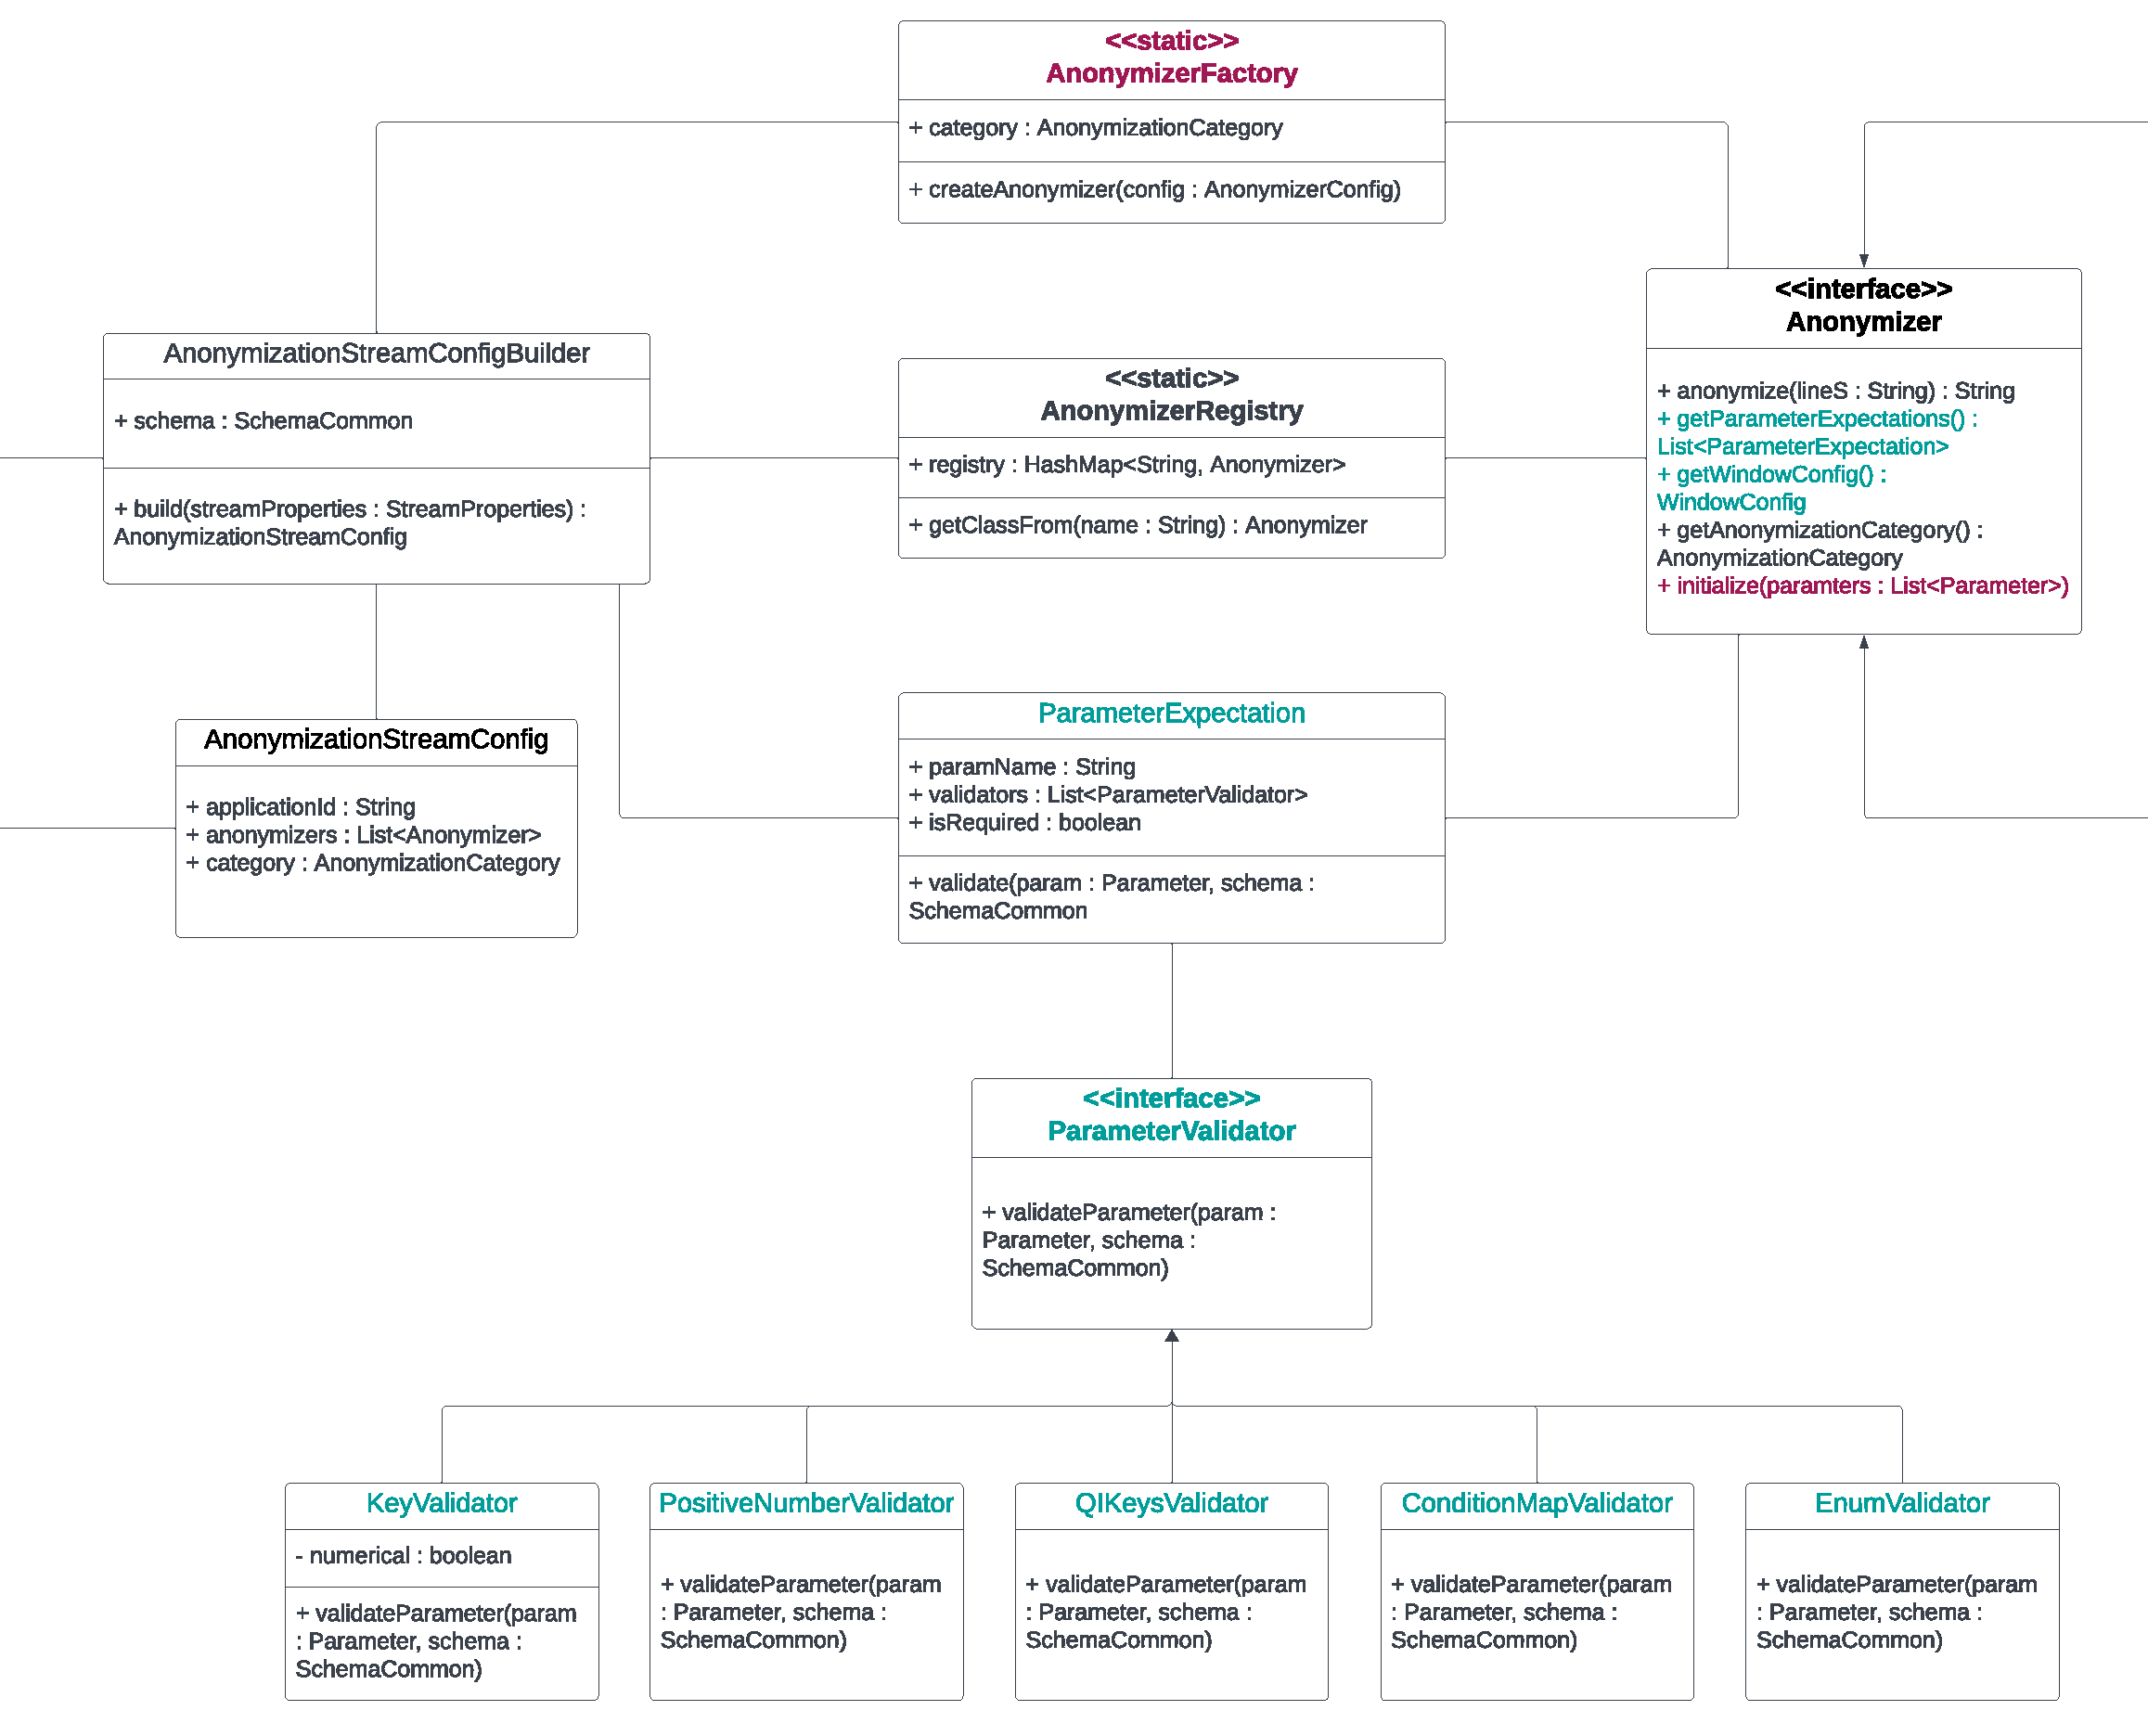
\includegraphics[width=0.85\pdfpagewidth]{img/Stream_Config_Builder.pdf}
   \end{adjustbox}
   \caption[Class diagram of the configuration builder component of \ac{DASH}]{Class Diagram of the stream configuration builder component and its corroborators responsible for validating (highlighted in teal) and instantiating (highlighted in red) individual anonymization stream configurations. It connects on the right to the individual anonymizers and on the left to the managing component of \ac{DASH}. The full diagram can be found in the Appendix in Figure \ref{fig:full_class_diagram}\label{fig:stream_config_builder}}
\end{figure}

Following the initialization, for an anonymization stream with attribute-based anonymizers their windowing strategy is validated. As many anonymizers can be included in one stream, but only one windowing technique is applied per stream, it must be ensured that all anonymizers have the same window configuration. \par
Finally, a new \texttt{AnonymizationStreamConfig} is created and returned, which includes the stream's name, its anonymizers, and the anonymization category. \par
If any of these validations fail \ac{DASH} will not proceed to running any streams, instead the setup phase will fail and an extensive log is output to the Data Officer to aid in fixing the setup mistakes. 

\subsection{Centralizing Stream Management\label{sec:stream_manager}}
The \texttt{StreamManager} functions as the operational extension of the Data Officer within \ac{DASH}. This entity centralizes all operations and handles both internal and external communications within \ac{DASH}. Take a look at Figure \ref{fig:stream_manager} for the Class Diagram. In the diagram, all green highlighted functionalities are directly administrable by the Data Officer. 

\begin{figure}[ht]
   \begin{adjustbox}{center}
      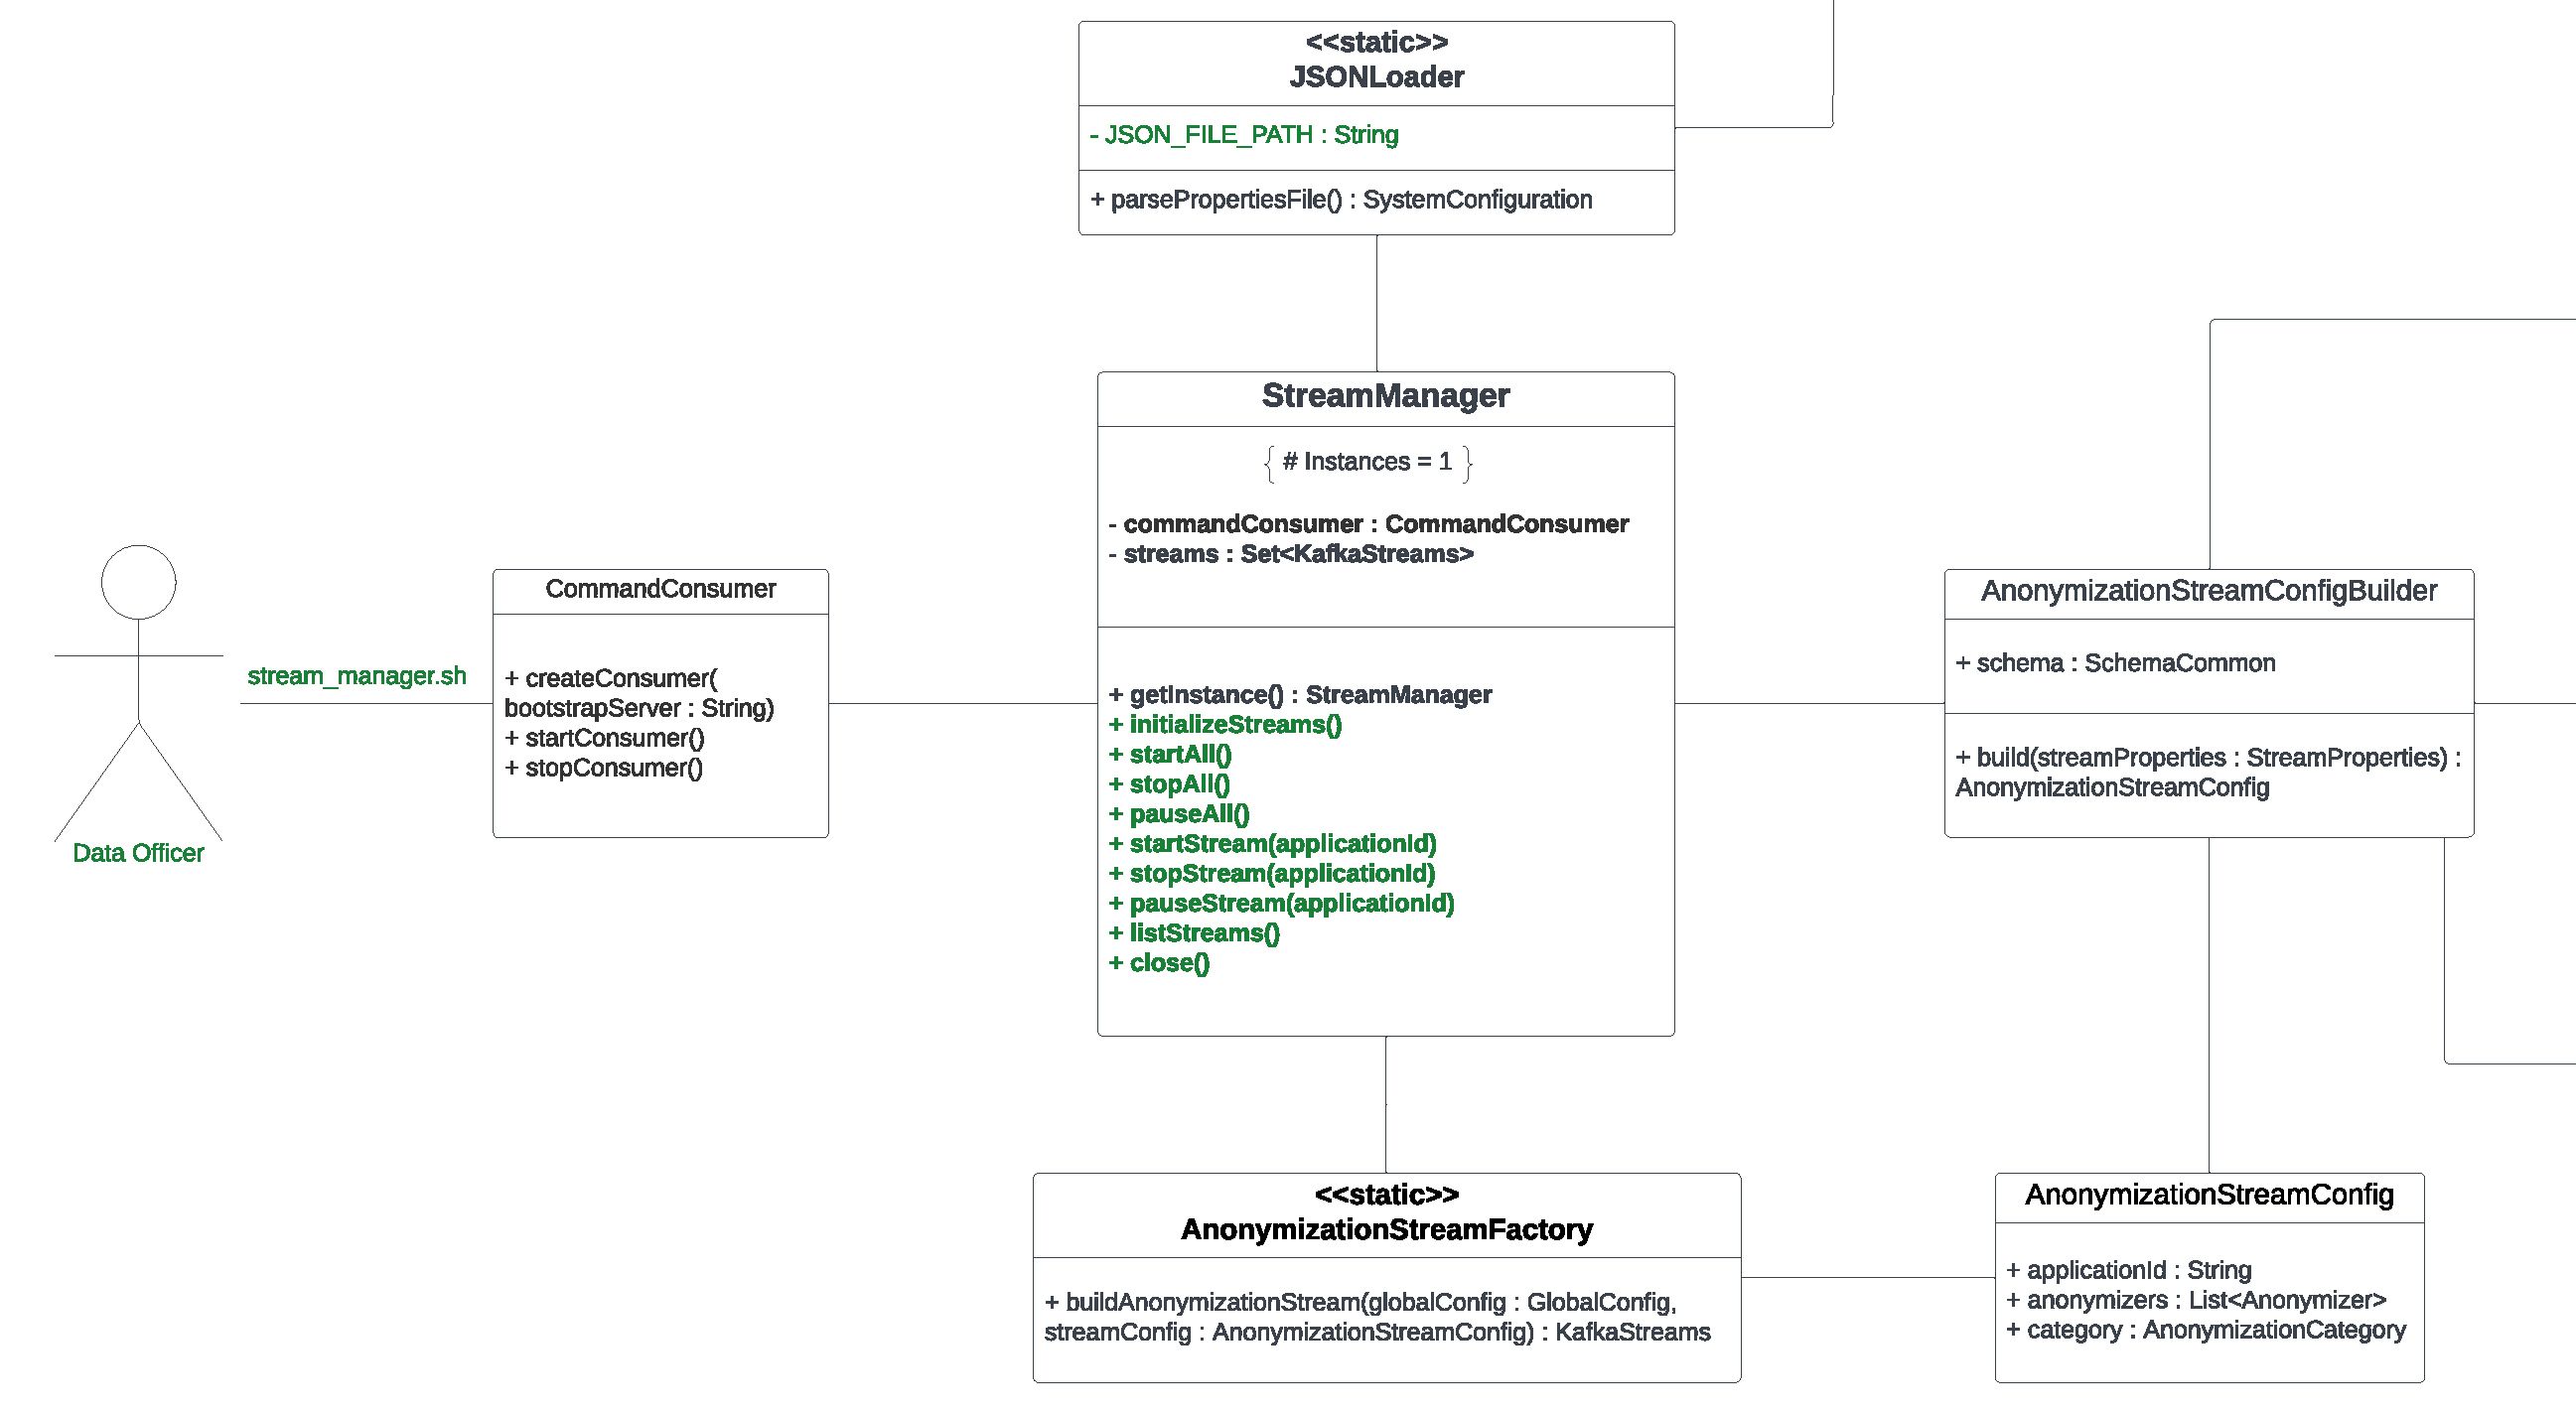
\includegraphics[width=0.85\pdfpagewidth]{img/Stream_Manager.pdf}
      \end{adjustbox}
      \caption{The central component of DASH illustrated in a UML Class Diagram. All green highlighted functionalities are directly administered by the Data Officer. It connects at the top to the rest of the requirements parsing component, and to the right to the stream configuration building component. The full diagram can be found in the Appendix in Figure \ref{fig:full_class_diagram}\label{fig:stream_manager}}
\end{figure}

In the center is the \texttt{StreamManager}. The constraint notation beneath the class name in Figure \ref{fig:stream_manager} denotes the Singleton pattern, ensuring a single instance is instantiated and globally accessible within the system. The Data Officer invokes system actions through the \texttt{stream\_manager.sh} shell script, located at the system's root directory. This opens up a command line, which internally creates (in true Kafkaesque fashion) a Kafka Producer. Commands issued during the session are produced to a designated 'commands' topic. The CommandConsumer within DASH subscribes to this topic and forwards the commands to the StreamManager. The commands encompass initialization, starting, pausing, and stopping of all or individual streams, and terminating \ac{DASH}. Additionally, there is a help command, which is also invoked on wrong input, to aid the Data Officer in administering and a list command to monitor the running system.
The \texttt{JSONLoader} as well as the \texttt{AnonymizationStreamConfigBuilder} and the \texttt{AnonymizationStreamConfig} are previously introduced components, serving specific functions in stream configuration and setup. The \texttt{AnonymizationStreamFactory} handles the creation and configuration of the anonymization streams on the Kafka side. The global config defines the source Kafka Stream. The tuples then are forwarded to the stream specified in the \texttt{AnonymizationStreamConfig}. Subsequently, tuples are anonymized according to their category, as determined by the configuration. The anonymization itself is executed by the function within the anonymizer, which is specified by the configuration. In the case of an attribute-based stream, the stream is first windowed according to the specification, aggregated, and then forwarded as a collection of tuples to the anonymizers. All streams can contain multiple anonymizers, which process the data sequentially. This means that the output of the first anonymizer will be the input of the second anonymizer and so on.\par
Ultimately, the system publishes the anonymized tuples to a newly created topic within Kafka. Its naming convention is '\{source\_stream\_name\}-\{application\_id\}'. From here they exist in the Kafka server and can be consumed from outside \ac{DASH}. In combination with the aforementioned RBAC system, these newly produced topics can be restricted to be only consumable by users who are assigned to a certain role. 

\section{Data Pipeline}
To facilitate the development and evaluation of \ac{DASH} and \ac{RBAC} mechanisms within Kafka, we implemented a data pipeline. It encompasses a data generator feeding data into a custom Kafka Connector. Within Kafka, the data is anoynmized and distributed into multiple role-restricted output data streams. These are read by Kafka Consumers. Figure \ref{fig:data_pipeline} depicts the flow of data from the source to the destination as indicated by the blue arrows. Each component is associated with its respective detailed explanation in the indicated sections. 

\begin{figure}[ht]
   \begin{tikzpicture}[node distance=2.3cm, auto, trim left=-0.25cm]
      \tikzstyle{system} = [rectangle, draw, rounded corners, text width=5em, text centered, minimum height=3em]
      \tikzstyle{arrow} = [thick,->,>=stealth]

      \node [system] (datagen) {Data Generator};
      \node [system, right=of datagen] (kafkacon) {Kafka Connector};
      \node [system, right=of kafkacon] (Kafka) {Kafka};
      \node [system, right=of Kafka] (kafkacons) {Kafka Consumers};

      \draw [arrow, color=dataBlue] (datagen) -- node[anchor=south] {\footnotesize{CSV data}} (kafkacon);
      \draw [arrow, color=dataBlue] (kafkacon) -- node[anchor=south] {\footnotesize{Struct data}} (Kafka);
      \draw [arrow, color=dataBlue] (Kafka) -- node[anchor=south, text width=2cm, text centered] {\footnotesize{Anonymized \\ structs}} (kafkacons);

      \node [above of=datagen, yshift=-0.5cm] (sec1) {Section \ref{sec:data_gen}};
      \node [above of=kafkacon, yshift=-0.5cm] (sec2) {Section \ref{sec:kafka_connector}};
      \node [above of=Kafka, yshift=-0.5cm] (sec3) {Section \ref{sec:dash}};
      \node [above of=kafkacons, yshift=-0.5cm] (sec4) {Section \ref{sec:kafka_consumer}};
      
      \draw [<-, color=black, dashed] (datagen.north) -- (sec1);
      \draw [<-, color=black, dashed] (kafkacon.north) -- (sec2);
      \draw [<-, color=black, dashed] (Kafka.north) -- (sec3);
      \draw [<-, color=black, dashed] (kafkacons.north) -- (sec4);
\end{tikzpicture}
\caption{Data Pipeline of the Implementation: The diagram shows the various components and their data flow, indicated by blue arrows, with references to the corresponding sections.}
\label{fig:data_pipeline}
\end{figure}
   
In this section, we will take a closer look at the components of the data pipeline outside of Kafka. It follows the flow of data beginning with the generator. 

\subsection{Data Generator\label{sec:data_gen}}
The data generator, developed in Python and accessible via a Jupyter Notebook \cite{jupyter_notebook}, is designed to simulate patient data for a German hospital specializing in diabetes care, as detailed in the Use Case Example (Section \ref{sec:anon_granularity}). Operating on a Python3 kernel, this generator utilizes modules such as Pandas \cite{pandas}, Numpy \cite{numpy}, and Faker \cite{faker} to create and manipulate CSV data. \par
The number of lines generated can be specified at the top of Data Generation section of the \texttt{dataGenerator.ipynb} notebook by adjusting the \texttt{nRows} value. A sample collection of data generated in this way with $nRows = 40$ is shown in the Appendix in Table \ref{tab:patient_data}. The script employs the Faker module for generating realistic yet fictitious personal data, such as names, addresses, and phone numbers. Additionally, a seed can be specified to easily reproduce the same data. \par
The data generator also ensures diversity in data by assigning gender, diagnosis, insurance companies, and other patient attributes based on realistic distributions and correlations. For instance, the genders Male and Female are assigned 48 percent of the time respectively for each entry, and 2 percent it assigned to Non-Binary. Similarly, it generates the diagnosis of Type 1 in nine percent of the cases, Type 2 in 89 percent, and Type 1.5 in the remaining two. An insurance company is randomly assigned to each entry according to their distribution in Germany. Height, weight, age, glucose, and HbA1C are randomly assigned from within a provided reasonable range. The medication is correlated with the diagnosis. \par
The generator's design allows for straightforward adjustments of data randomness, structure, and volume, which can be configured in the initial cell of the notebook.

\subsection{Kafka Connector\label{sec:kafka_connector}}
Since CSV files cannot be directly published to the Kafka network, it requires the use of a middleman, a Kafka Producer. This requirement is frequently encountered by Kafka users. This is where Kafka Connectors come into play. They alleviate this task of developing a Producer manually and transform the data for the user. There are many such Connectors available, but most are restricted by licenses that restrict their usage. Therefore, we developed our own Kafka Connector for CSV files. \par
Implementing a custom connector involves utilizing two key interfaces of the Kafka Connect framework: \texttt{SourceConnector} and \texttt{SourceTask}. The source connector class sets up the connection to Kafka. This includes setting the properties for the server, the security protocols, and the topic name that the connector should produce to. It also specifies the \texttt{SourceTask} class and how many instances of that class should run simultaneously.\par
The implemented task reads the CSV file located in a fixed location. Data is read into a buffer employing Java's \texttt{BufferedReader}. This buffer, containing a batch of lines, is then processed. Lines are extracted by detecting end-of-line characters '$\backslash$n' and '$\backslash$r'. The lines are converted into Kafka Structs with a predefined Schema that fits the data generated by the aforementioned Python script. Ultimately, the structs are produced to the specified topic in batches. \par
The connector is integrated with the Kafka server by compiling the Java code into a JAR file and transferring this file to Kafka's distribution data folder. Subsequently, it can be executed with the specified properties at runtime.

\subsection{Kafka Consumers\label{sec:kafka_consumer}}
In general, the terminal consumers included in the Apache Kafka distribution suffice for numerous implementations. It simply consumes the tuples from a specified topic. However, when implementing access control and simultaneously monitoring multiple data streams, the setup becomes laborious. \par
Consequently, a script was developed to instantiate consumers with predefined roles, including authentication, in a unified setup. It is set up with the specifications of the default \ac{DASH} configuration and writes the consumed tuples to the terminal. Unlike default terminal consumers that output data as plain text, custom consumers recognize the data structure and display it in a more aesthetically pleasing format. \par
The implementation details are available in the 'consumers' folder within the Kafka pipeline directory.


\section{Docker-based System Integration}
The systems developed, including Kafka, ZooKeeper, the \ac{RBAC} system, \ac{DASH}, the data generator, the source connector, and consumers, are designed to operate in conjunction. This ensemble forms a complete data pipeline, simulating data streams being anonymized in real-time. However, the simultaneous management of seven or more systems can be a fault-prone and tedious process, requiring the handling of numerous terminals and configurations. This is why we have opted early in the development process to unify building, deploying, and running all systems in containers using Docker \cite{docker}. \par
Docker facilitates the containerization of applications into standardized, executable components. This is achieved by allocating resources from the underlying hardware for use by the Docker engine. Atop this engine, within the container, developers can freely choose the operating system to build the application. The application within the container will then be runnable on any environment simplifying the deployment. \par
The integration of multiple containers is efficiently achieved through a 'Docker Compose' file. Each Docker container is specified as a service in the compose file. This is how our systems are unified and become executable in any environment with the simple command \texttt{Docker compose up} in the code folder of the repository (which can be found alongside all other artifacts, the thesis itself, and relevant literature in \url{https://github.com/TheRealHenri/master_thesis}).\par
The compose file is written in yaml and lists services e.g. containers followed by internal structures such as networks and Docker volumes. The latter can be used for persisting storage generated by and used by Docker containers. There are two types of volume storage: bind mounts point to the storage of the host system, Docker volumes on the other hand are completely managed by Docker. 
Each service represents a Docker container and consists of its specifications as shown in Code Fragment \ref{lst:docker_container}. 

\begin{lstlisting}[language=yaml, captionpos=b, caption={General structure of a docker compose file.}, label={lst:docker_container}]
   service_name:
      build: ./path/to/project 
      # alternatively: 
      image: 'dockerhub_link'
      networks:
         - network_name
      ports: 
         - internal_port:exposed_port
      depends_on:
         - other_service_name
      environment: 
         - variable_name: variable_value
      volumes: 
         - ./storage/path/locally:/docker/path1
         - docker-volume:/docker/path2
      command: executed_on_startup
   
   other_service_name: 
      ...
   
   networks: 
      network_name: 
         driver: driver_type
   
   volumes: 
      docker-volume:
\end{lstlisting}
   
For each service within Docker, the specification of either a build or an image is mandatory. The build refers to a project with its own Dockerfile. Images may be selected from Docker Hub \cite{dockerhub}. We use the \texttt{bitnami/zookeeper:3.8.2} image for zookeeper and the \texttt{bitnami/kafka:3.5.1} image for kafka. The rest of our systems were developed from scratch and included a Dockerfile with the necessary build information. \par
In the docker compose, we specify a network for all containers to use called simply 'kafka\_network'. This allows containers within the network to communicate with each other by service name instead of IP address. In addition, communication necessitates exposed ports; without these, inter-container is not possible. Ports exposed by the application running inside a container need to be mapped to ports accessible from the outside. For instance, Kafka exposes the communication port 9092 to its clients and on port 8083 with its connectors. The communication between Kafka and Zookeeper occurs on port 2021. We have set up the data generator to run on a web socket on port 8888, so if someone using the system wants to change the way data is generated, the person can do it during runtime with a user interface in the browser at \texttt{localhost:8888}. \par
Dependencies among containers are also managed through the Docker Compose file. For instance \ac{RBAC}, \ac{DASH}, and the Kafka Connector are dependent on a running Kafka server. Kafka in turn is dependent on a running ZooKeeper instance. These dependencies can be specified by simply adding the name in the 'depends\_on' section of the compose. Furthermore, since version 3 of compose, the status of the dependent container can be specified as well. We require the data pipeline build process to be finished successfully before starting the Kafka connector. This better allocates resources at runtime by not spending it on processes that would have to wait for others later on. \par
Environment variables correspond to configuration parameters within the system. Commonly, there is a set of parameters available for images from Dockerhub. In the case of the Kafka image, several parameters have to be set. For one the listeners dictate the protocols used for internal and external communication with the server. Additionally, the zookeeper communication is specified as well. In our docker compose we emulate a distributed event store. For this, we run the Kafka server on three different brokers. Each broker is assigned its container, they differentiate in their port mappings as well as, crucially, their broker ID environment variable. All clients and connectors specify all three brokers as their bootstrap server e.g. \texttt{bootstrapServer=kafka1:9092,kafka2:9093,kafka3:9094}. \par
We utilize Docker volumes for data storage. As intended by Docker we use bind mounts for data we specify on the host system like the Data Officer's anonymization requirements, Kafka Connector's configuration, and the \ac{RBAC} database. For data shared between containers, we use specific Docker volumes managed by Docker. For example, the data generator produces a CSV file used by the Kafka Connector. Produced logs are also stored in Docker. \par
Finally, a command can be specified to be executed upon completion of the build process. Calling \texttt{docker compose up} starts up all containers and executes the specified command. The \ac{RBAC} system opens a shell for the \ac{CLI}, while the Kafka Connector is started up with a shell script. \par
Ultimately, Docker is configured to initially launch ZooKeeper, followed by the Kafka server with three operational brokers for load balancing. In the meantime, data is generated. Upon completion, the Kafka Connector, the \ac{RBAC} system, and \ac{DASH}. The generated data is fed through the Connector into \ac{DASH} and produced to the anonymized streams. This entire process is executable through a single command in one terminal, provided Docker is installed on the host system. 